\documentclass[]{book}

%These tell TeX which packages to use.
\usepackage{array,epsfig}
\usepackage{amsmath}
\usepackage{amsfonts}
\usepackage{amssymb}
\usepackage{amsxtra}
\usepackage{amsthm}
\usepackage{mathrsfs}
\usepackage{color}
\usepackage{mathtools}
\usepackage{hyperref}
\usepackage{cleveref}

%Here I define some theorem styles and shortcut commands for symbols I use often
\theoremstyle{definition}
\newtheorem{defn}{Definition}
\newtheorem{thm}{Theorem}
\newtheorem{cor}{Corollary}
\newtheorem*{rmk}{Remark}
\newtheorem{lem}{Lemma}
\newtheorem*{joke}{Joke}
\newtheorem{ex}{Example}
\newtheorem*{soln}{Solution}
\newtheorem{prop}{Proposition}

\newcommand{\lra}{\longrightarrow}
\newcommand{\ra}{\rightarrow}
\newcommand{\surj}{\twoheadrightarrow}
\newcommand{\graph}{\mathrm{graph}} \newcommand{\bb}[1]{\mathbb{#1}}
\newcommand{\Z}{\bb{Z}} \newcommand{\Q}{\bb{Q}} \newcommand{\R}{\bb{R}}
\newcommand{\C}{\bb{C}} \newcommand{\N}{\bb{N}} \newcommand{\M}{\mathbf{M}}
\newcommand{\m}{\mathbf{m}} \newcommand{\MM}{\mathscr{M}}
\newcommand{\HH}{\mathscr{H}}
\newcommand{\Om}{\Omega}
\newcommand{\Ho}{\in\HH(\Om)}
\newcommand{\bd}{\partial}
\newcommand{\del}{\partial}
\newcommand{\bardel}{\overline\partial}
\newcommand{\textdf}[1]{\textbf{\textsf{#1}}\index{#1}}
\newcommand{\img}{\mathrm{img}}
\newcommand{\ip}[2]{\left\langle{#1},{#2}\right\rangle}
\newcommand{\inter}[1]{\mathrm{int}{#1}}
\newcommand{\exter}[1]{\mathrm{ext}{#1}} \newcommand{\cl}[1]{\mathrm{cl}{#1}}
\newcommand{\ds}{\displaystyle}
\newcommand{\vol}{\mathrm{vol}} \newcommand{\cnt}{\mathrm{ct}}
\newcommand{\osc}{\mathrm{osc}} \newcommand{\LL}{\mathbf{L}}
\newcommand{\UU}{\mathbf{U}} \newcommand{\support}{\mathrm{support}}
\newcommand{\AND}{\;\wedge\;}
\newcommand{\OR}{\;\vee\;}
\newcommand{\Oset}{\varnothing}
\newcommand{\st}{\ni}
\newcommand{\wh}{\widehat}
\newcommand{\XX}{\mathbf{X}} \newcommand{\YY}{\mathbf{Y}}
\newcommand{\BB}{\mathbf{B}}
\renewcommand{\AA}{\mathbf{A}}
\newcommand{\VV}{\mathbf{V}}
\newcommand{\DD}{\mathbf{D}}
\newcommand{\EE}{\mathbf{E}}
\newcommand{\ZZ}{\mathbf{Z}}
\newcommand{\RR}{\mathbf{R}}
\newcommand{\QQ}{\mathbf{Q}}
\newcommand{\yy}{\mathbf{y}}
\newcommand{\cc}{\mathbf{c}}
\newcommand{\zz}{\mathbf{z}}
\newcommand{\TT}{\mathcal{T}} 
\newcommand{\WW}{\mathbf{W}}
\newcommand{\II}{\mathbf{I}}
\newcommand{\ridge}{\textsf{ridge}}
\newcommand{\lasso}{\textsf{lasso}}

\DeclareMathOperator*{\argmax}{arg\,max}
\DeclareMathOperator*{\argmin}{arg\,min} \DeclareMathOperator*{\Cov}{Cov}
\DeclareMathOperator*{\EPE}{EPE} \DeclareMathOperator*{\Var}{Var}
\DeclareMathOperator*{\Bias}{Bias} \DeclareMathOperator*{\tr}{trace}
\DeclareMathOperator*{\RSS}{RSS} \DeclareMathOperator*{\WRSS}{WRSS}
\DeclareMathOperator*{\MSE}{MSE} \DeclareMathOperator*{\diag}{diag}


%Pagination stuff.
\setlength{\topmargin}{-.3 in}
\setlength{\oddsidemargin}{0in}
\setlength{\evensidemargin}{0in}
\setlength{\textheight}{9.in}
\setlength{\textwidth}{6.5in}
\pagestyle{empty}



\begin{document}


\begin{center}
	{\Large Elements of Statistical Learning, Solutions}\\
	Marios\\ %You should put your name here
\end{center}

\vspace{0.2 cm}


\section*{Exercises for Section 2}

\begin{enumerate}
	\item\label{ex:k-classes} Suppose each of $K$-classes has an associated
	target $t_k$, which is a vector of all zeros, except a one in the $k$th
	position. Show that classifying to the largest element of $\hat{y}$ amounts
	to choosing the closest target, $\min_k\|t_k-\hat{y}\|$, if the elements of
	$\hat{y}$ sum to one.
	\begin{soln}
		\newcommand{\normone}[1]{\sum_{i\ne #1}|\hat{y}_i|+|1-\hat{y}_{#1}|} Let
		$k^*=\argmax_k \hat{y}_k$ and suppose that there is $k'\le k^*$ such
		that $\|t_{k'}-\hat{y}\| < \|t_{k^*}-\hat{y}\|$.
		\begin{itemize}
			\item $\ell_1$ norm. It holds that
			      $\|t_k-\hat{y}\|_1=\sum_i|t_{k,i}-\hat{y}_i|=\sum_{i\ne
					      k}|\hat{y}_i|+|1-\hat{y}_k|$. Hence, we get
			      \begin{equation}\label{2.1-inequality}
				      \normone{k'} < \normone{k^*}\Rightarrow |\hat{y}_{k^*}|-|1-\hat{y}_{k^*}|
				      < |\hat{y}_{k'}|-|1-\hat{y}_{k'}|.
			      \end{equation}
			      But the function $f(y)=|y|-|1-y|$ is increasing in $[0,1]$
			      hence~\Cref{2.1-inequality} implies that
			      $\hat{y}_{k^*}<\hat{y}_{k'}$, reaching a contradiction.
			\item $\ell_2$ norm. Similarly, we get that
			      $\hat{y}_{k^*}(1-\hat{y}_{k^*})<\hat{y}_{k'}(1-\hat{y}_{k'})$
			      and since the function $f(y)=y(1-y)$ is increasing in $[0,1]$,
			      we get that $\hat{y}_{k^*}<\hat{y}_{k'}$, reaching a
			      contradiction.
		\end{itemize}
	\end{soln}

	\item\label{ex:exact-distribution} Show how to compute the Bayes decision
	boundary for the simulation example in Figure 2.5.
	\begin{soln}
		If we know the exact probability distribution $\Pr[G,X]$,
		$X\in\mathbb{R}^p$, $G\in \mathcal{G}=\{B,O\}$, then we can probably
		also derive $f(X)=\Pr[B|X]=\Pr[B,X]/\Pr[X]$, namely the probability that
		$X$ maps to blue in reality. This assume that we also know $\Pr[X]$
		which is not necessary. Of course, $\Pr[O|X]=1-\Pr[B|X]$. So now, all we
		have to do is to check for each $x\in\mathbb{R}^p$, whether $f(x)>1/2$.
		For the case where $x\in\mathbb{R}$, this is trivial. We simply solve
		the equation $f(x)=1/2$. This also hold in general. So the points (in
		$\mathbb{R}$), the line (in $\mathbb{R}^2$), and the $(p-1)$-dimensional
		hyperplane (in $\mathbb{R}^p$), is the solution to the equation
		$f(x)=\Pr[B|X]=1/2$. See Figure~\ref{fig:exercise2.2} for another
		example.

		\begin{figure}[ht]
			\label{fig:exercise2.2}
			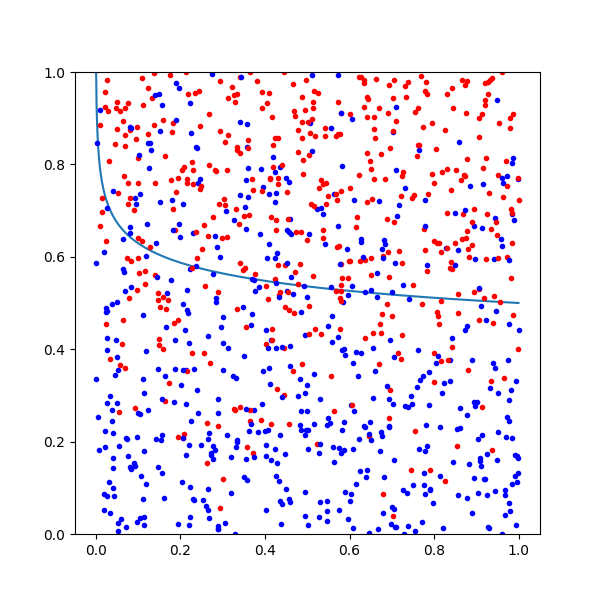
\includegraphics[width=8cm]{../plots/ex22.png}
			\centering
			\caption{In this example we have computed the Bayes decision
			boundary when $X\sim U(0,1)^2$ and
			$\Pr[Y=\text{red}|X]=X_1^{1/10}X_2$. Therefore, the line is the
			solution to the equation $X_1^{1/10}X_2=1/2$.}
		\end{figure}
	\end{soln}

	\item\label{ex:eq2.24} Derive equation 2.24. Consider $N$ data points
	uniformly sampled in a $p$-dimensional unit ball centered at the origin.
	Show that the median distance from the origin to the closest data point is
	given by the expression $$d(p,N)=\left(1-\frac{1}{2}^{1/N}\right)^{1/p}.$$
	\begin{soln}
		We start with the cumulative distribution function (CDF) of the distance
		of a random point from the origin. The volume of a $p$-dimensional ball
		of radius $d$ is $V_p(d)=c_pd^p$, where $c_p$ is a value that does not
		depend on $d$. Therefore,
		\begin{equation}\tag{First trick to remember}
			F_D(d)=\Pr[D\le d]=\frac{V_p(d)}{V_p(1)}=d^p.
		\end{equation}
		Now it is useful to compute the CDF of the distance of the closest point
		$C=\min_{i\in[N]} D_i$. We have that
		\begin{equation}
			\begin{split}
				F_C(d) &= \Pr[C\le d] \\
				&= 1-\Pr[C\ge d] \\
				&= 1-\Pr\left[\min_{i\in[N]} D_i \ge d\right] \\
				&= 1-\Pr[\forall i\in[N], D_i \ge d] \\
				&= 1-\prod_{i\in[N]}\Pr[D_i \ge d] \\
				&= 1-\Pr[D \ge d]^N \\
				&= 1-(1-\Pr[D \le d])^N \\
				&= 1-(1-d^p)^N.
			\end{split}
		\end{equation}
		By definition, the median $m$ is defined as $F_C(m)=1/2$. Hence, we get
		that $(1-m^p)^N=1/2$ and solving for $m$, we get
		\[m=\left(1-\frac{1}{2}^{1/N}\right)^{1/p}.\]
	\end{soln}

	\item\label{ex:multi-normal} Consider inputs drawn from a spherical
	multinormal distribution $X\sim N(0,\mathbf{I}_p)$. The squared distance
	from any sample point to the origin has a $\chi_p^2$ distribution with mean
	$p$. Consider a prediction point $x_0$ drawn from this distribution, and let
	$a=x_0/\|x_0\|$ be an associated unit vector. Let $z_i=a^Tx_i$ be the
	projection of each of the training points on this direction.

	Show that the $z_i$ are distributed according to $N(0,1)$ with expected
	squared distance from the origin $1$, while the target point has expected
	squared distance $p$ from the origin.

	\begin{soln}
		We use the fact that for any $a\in\mathbb{R}^p$, if $x\sim
			N(0,\mathbf{I}_p)$, then $a^Tx\sim
			N\left(\sum_ja_j\mu_j,\sum_ja_j^2\sigma_j^2\right)$, where
		$\mu_j=E(x_j)$ and $\sigma_j=V(x_j)$ and $j\in[p]$. Since
		$\sigma_j=1$ and $\mu_j=0$, we get that $a^Tx\sim
			N\left(0,\sum_ja_j^2\right)$. Given that $\|a\|$ is a unit vector,
		we get that $a^Tx\sim N\left(0,1\right)$. Hence
		$|z|=|a^Tx|\sim\chi_1^2$ and $E[|z|]=1$.
	\end{soln}

	\item\label{ex:eq2.27} Suppose that we know that the true relationship
	between $Y$ and $X$ is linear,
	\begin{equation}
		Y=X^T\beta+\varepsilon, \tag{2.26}
	\end{equation}
	where $\varepsilon\sim N(0,\sigma^2)$ and we fit the model by least squares
	to the training data. For an arbitrary test point $x_0$, we have $\hat
		y_0=x_0^T\hat\beta$, which can be written as $\hat y_0=x_0^T\beta +
		\sum_{i-1}^N\ell_i(x_0)\varepsilon_i$, where $\ell_i(x_0)$ is the $i$th
	element of $\XX(\XX^T\XX)^{-1}x_0$. Show that
	\[
		\EPE(x_0)=\sigma^2+E_\TT x_0^T(\XX^T\XX)^{-1}x_0\sigma^2+0^2 \tag{2.27},\]
	where you can use the fact that for any $\XX$,
	\[\Cov[\hat \beta]=(\XX^T\XX)^{-1}\sigma^2. \label{eq:cov}\tag{3.8}\]
	Additionally, suppose $N$ is large and $\TT$ were selected at random.
	Assuming $E(X)=0$, then $\XX^T\XX\to N\Cov(X)$. Show that
	\begin{equation*}
		\begin{split}
			E_{x_0}\EPE(x_0) &\approx E_{x_0}x_0^T \Cov[X]^{-1}x_0\sigma^2/N + \sigma^2\\
			&=\tr[\Cov[X]^{-1}\Cov[x_0]]\sigma^2/N+\sigma^2 \\
			&=\sigma^2(p/N)+\sigma^2.
		\end{split}\tag{2.28}
	\end{equation*}
	Make use of the cyclic property of the trace operator ($\tr(AB)=\tr(BA)$),
	and its linearity (which allows us to interchange the order of trace and
	expectation).

	\begin{soln}
		{ \newcommand{\Exp}{E_{\TT,\varepsilon}} In the first question, the test
			point $x_0$ is arbitrary and not sampled from the distribution. Thus
			the randomness is only over:
			\begin{itemize}
				\item the samples $\TT$,
				\item the error $\varepsilon$.
			\end{itemize}
			In the second part, we also sample $x_0$ and hence we consider the
			expectation of $\EPE(x_0)$.
			\begin{enumerate}
				\item We start by showing that the expected prediction error
				      equals the sum of the variance of the system, the variance
				      of the model and the squared bias of the model:
				      \begin{equation*}
					      \begin{split}
						      \EPE(x_0) &= \Exp[(y_0-\hat y_0)^2] \\
						      &= \Exp[y_0^2-2y_0\hat y_0 + \hat y_0^2] \\
						      &= \Exp[y_0^2]-2\Exp[y_0\hat y_0] + \Exp[\hat y_0^2] \\
						      &= \Exp[y_0^2]-2x_0^T\beta\Exp[\hat y_0] + \Exp[\hat y_0^2] \\
						      &= \Exp[y_0^2]\boxed{-\Exp[y_0]^2+\Exp[y_0]^2}-2x_0^T\beta\Exp[\hat y_0] + \Exp[\hat y_0^2] - \boxed{\Exp[\hat y_0]^2 + \Exp[\hat y_0]^2} \\
						      &= \Var[y_0] + \Var[\hat y_0] + \left(\Exp[\hat y_0]-x_0^T\beta\right)^2,
					      \end{split}
				      \end{equation*}
				      where the third line follows from the fact that
				      \[\Exp[y_0\hat y_0]=\Exp[(x_0^T\beta+\varepsilon)\hat
						      y_0]=x_0^T\beta\Exp[\hat y_0]+\Exp[\varepsilon\hat
						      y_0]\] and $\Exp[\varepsilon\hat
						      y_0]=\Exp[\varepsilon]\Exp[\hat y_0]=0$, since
				      $\varepsilon$ is independent from $\hat y_0$. Now,
				      we have that $\Var[y_0]=\sigma^2$. Moreover,
				      \begin{equation}
					      \begin{split}
						      \Exp[\hat y_0] &= \Exp\left[x_0^T\beta + \sum_{i-1}^N\ell_i(x_0)\varepsilon_i\right] \\
						      &= x_0^T\beta + \sum_{i-1}^N\Exp[\ell_i(x_0)\varepsilon_i] \\
						      &= x_0^T\beta + \sum_{i-1}^N\Exp[\ell_i(x_0)]\Exp[\varepsilon_i] \\
						      &= x_0^T\beta,
					      \end{split}
				      \end{equation}
				      since $\varepsilon_i$ is independent of $x_0$ and $\XX$.
				      Hence, $\Bias(\hat y_0)=\left(\Exp[\hat
						      y_0]-x_0^T\beta\right)=0$. Last, we want to calculate the
				      variance of our prediction $\Var[\hat y_0]$. We have
				      \begin{equation}
					      \begin{split}
						      \Var[\hat y_0] &= \Var[x_0^T\hat\beta] \\
						      &= x_0^T\Cov[\hat\beta]x_0 \\
						      &= x_0^T(\XX^T\XX)^{-1}\sigma^2x_0,
					      \end{split}
				      \end{equation}
				      where the last line comes from~\cref{eq:cov}.
				\item Now we have that
				      \begin{equation}
					      \begin{split}
						      E_{x_0}\EPE(x_0) &\approx E_{x_0}[x_0^T \Cov[X]^{-1}x_0]\sigma^2/N + \sigma^2 \\
						      &= E_{x_0}[\tr[x_0^T \Cov[X]^{-1}x_0]]\sigma^2/N + \sigma^2 \\
						      &= E_{x_0}[\tr[\Cov[X]^{-1}x_0x_0^T]]\sigma^2/N + \sigma^2 \\
						      &= \tr[E_{x_0}[\Cov[X]^{-1}x_0x_0^T]]\sigma^2/N + \sigma^2 \\
						      &= \tr[\Cov[X]^{-1}E_{x_0}[x_0x_0^T]]\sigma^2/N + \sigma^2 \\
						      &= \tr[\Cov[X]^{-1}\Cov[x_0]]\sigma^2/N + \sigma^2 \\
						      &= \tr[\mathbf{I}_p]\sigma^2/N + \sigma^2 \\
						      &= p\sigma^2/N + \sigma^2
					      \end{split}
				      \end{equation}
			\end{enumerate}
		} We see that the function
		$f(p)=E_{x_0}\EPE(x_0)=\sigma^2(p/N)+\sigma^2$ increases linearly with
		$p$, with slope $f'(p)=\sigma^2/N$. Hence as long as we have
		sufficiently many samples $N$ this increase becomes negligible. In other
		words, even if we have a lot of dimensions, the expected $\EPE$ remains
		constant. Of course, the reason is that we imposed heavy restrictions on
		the class of models being fitted.
	\end{soln}

	\item\label{ex:2.6} Consider a regression problem with inputs $x_i$ and
	outputs $y_i$, and a parameterized model $f_\theta(x)$ to be fit by least
	squares. Show that if there are observations with \emph{tied} or
	\emph{identical} values of $x$, then the fit can be obtained from a reduced
	weighted least squares problem.

	\begin{soln}
		The weighted least squares problem is defined as the problem of
		minimizing the value
		\[\WRSS\nolimits_{(x_i,y_i,w_i)}(\beta)=\sum_{i=1}^Nw_i(y_i-\hat
			f_\beta(x_i))^2.\] It generasizes $\RSS$ since by setting $w_i=1$ we
		get the $\RSS$. The idea behind $\WRSS$ is that some pairs
		$(x_i,y_i)$ may have errors and some may be more accurate. By giving
		them weights, we reward the more accurate ones and we penalize the
		less accurate.

		A reduced least squares problem is one that uses fewer observations than
		available; $N'<N$.

		Suppose that we have $N$ observations $(x_i,y_i)$ with some of them
		sharing the same $x_i$. Suppose we have $N'$ distinct $x_i$s and for
		each distinct $x_i$, we have $N_i$ observations, so
		$N=\sum_{i=1}^{N'}N_i$. We wish to compute the value $\argmin_\beta
			\RSS(\beta)$. We will show that
		\[\argmin_\beta \RSS\nolimits_{(x_i,y_i)}(\beta)=\argmin_\beta
			\WRSS\nolimits_{(x_i,\overline y_i,N_i)}(\beta).\] We have{
				\newcommand{\fx}{\hat f_\beta(x_i)}
				\newcommand{\fs}{\hat f^2_\beta(x_i)}
				\begin{equation}
					\begin{split}
						\argmin_\beta \RSS\nolimits_{(x_i,y_i)}(\beta) &=
						\argmin_\beta\sum_{i=1}^N(y_i-\fx)^2 \\
						&= \argmin_\beta\sum_{i=1}^{N'}\sum_{j=1}^{N_i}(y_i-\fx)^2 \\
						&= \argmin_\beta\sum_{i=1}^{N'}\sum_{j=1}^{N_i}(y_i^2-2y_i\fx + \fs) \\
						&= \argmin_\beta\sum_{i=1}^{N'}\sum_{j=1}^{N_i}(-2y_i\fx + \fs) \\
						&= \argmin_\beta\sum_{i=1}^{N'}(-2N_i\overline y_i\fx + N_i\fs)\\
						&= \argmin_\beta\sum_{i=1}^{N'}N_i(-2\overline y_i\fx + \fs)\\
						&= \argmin_\beta\sum_{i=1}^{N'}N_i(\overline y_i^2-2\overline y_i\fx + \fs)\\
						&= \argmin_\beta\sum_{i=1}^{N'}N_i(\overline y_i-\fx)^2 \\
						&= \argmin_\beta\WRSS\nolimits_{(x_i,\overline y_i,N_i)}(\beta),
					\end{split}
				\end{equation}}
		where the fourth and the seventh lines come from the fact that for any
		function $f$ and $c\in\mathbb R$, it holds that $\argmin_\beta
			(f(\beta)+c)=\argmin_\beta{f(\beta)}$.
	\end{soln}

	\item Suppose we have a sample of $N$ pairs $x_i,y_i$ drawn i.i.d from the
	      distribution characterized as follows:
	      \begin{itemize}
		      \item[] $x_i\sim h(x)$, the design density
		      \item[] $y_i=f(x_i)+\varepsilon_i$, $f$ is the regression function
		      \item[] $\varepsilon_i\sim(0,\sigma^2)$ (mean zero, variance
			      $\sigma^2$)
	      \end{itemize}
	      We construct an estimator for $f$ \emph{linear} in the $y_i$,
	      \[\hat f(x_0)=\sum_{i=1}^N\ell_i(x_0;\mathcal{X})y_i,\] where the
	      weights $\ell_i(x_0;\mathcal{X})$ do not depend on the $y_i$, but do
	      depend on the entire training sequence of $x_i$, denoted here by
	      $\mathcal{X}$.
	      \begin{enumerate}
		      \item Show that the linear regression and $k$-nearest-neighbor
		            regression are members of this class of estimators. Describe
		            explicitly the weights $\ell_i(x_0;\mathcal{X})$ in each of
		            these cases.
		      \item Decompose the conditional mean-squared error
		            \[E_{\mathcal{Y}|\mathcal{X}}(f(x_0)-\hat f(x_0))^2\] into a
		            conditional squared bias and a conditional variance
		            component. Like $\mathcal{X}$, $\mathcal{Y}$ represents the
		            entire training sequence of $y_i$.
		      \item Decompose the mean-squared error
		            $E_{\mathcal{X,Y}}(f(x_0)-\hat f(x_0))^2$ into a squared
		            bias and a variance component.
		      \item Establish a relationship between the squared biases and
		            variances in the above two cases.
	      \end{enumerate}

	      \begin{soln}{ \renewcommand{\XX}{\mathcal{X}}
			      \renewcommand{\YY}{\mathcal{Y}}
			      \begin{enumerate}
				      \item For linear regression, we have that $\hat f(x_0) =
					            x^T(\XX^T\XX)^{-1}\XX
					            y=\sum_{i=1}^N\ell_i(x_0;\XX)y_i$, where
				            $\ell_i(x_0;\XX)$ is the $i$th element of the
				            vector $x^T(\XX^T\XX)^{-1}\XX$. For the
				            $k$-nearest neighbor, we have that
				            $\ell_i(x_0;\XX)=\frac{1}{k}I(x_i\in
					            N_k(x_0,\XX))$, where $N_k(x_0,\XX)$ is the set
				            of the $k$ closest points to $x_0$.

				      \item We have that
				            \begin{equation}
					            \begin{split}
						            E_{\YY/\XX}[(f(x_0)-\hat f(x_0))^2]
						            &= E_{\YY/\XX}[f^2(x_0)-2f(x_0)\hat f(x_0)+\hat f^2(x_0)] \\
						            &= \Var\nolimits_{\YY/\XX}(f(x_0)) + \Var\nolimits_{\YY/\XX}(\hat f(x_0)) +
						            E_{\YY/\XX}[(f(x_0)-\hat f(x_0))]^2 \\
						            &= \Var\nolimits_{\YY/\XX}(f(x_0)) + \Var\nolimits_{\YY/\XX}(\hat f(x_0)) +
						            \Bias\nolimits_{\YY/\XX}[\hat f(x_0)]^2 \\
						            &= \Var\nolimits_{\YY/\XX}(\hat f(x_0)) +
						            \Bias\nolimits_{\YY/\XX}[\hat f(x_0)]^2
					            \end{split}
				            \end{equation}
				            since $f(x_0)$ does not have any randomness.
				      \item Similarly,
				            \begin{equation}
					            \begin{split}
						            E_{\YY,\XX}[(f(x_0)-\hat f(x_0))^2]
						            &= \Var\nolimits_{\YY,\XX}(\hat f(x_0)) +
						            \Bias\nolimits_{\YY,\XX}[\hat f(x_0)]^2.
					            \end{split}
				            \end{equation}
				      \item We have that
				            \[\Var\nolimits_{\YY,\XX}(\hat f(x_0)) = E_{\XX\sim
					            h}[\Var\nolimits_{\YY,\XX}(\hat f(x_0))]\]
				            \[\Bias\nolimits_{\YY,\XX}(\hat f(x_0)) = E_{\XX\sim
					            h}[\Bias\nolimits_{\YY,\XX}(\hat f(x_0))]\]
			      \end{enumerate}}
	      \end{soln}

	      \item\label{ex:2.8} Compare the classification performance of linear
	      regression and $k$-nearest neighbor classification on the
	      \texttt{zipcode} data. In particular, consider only the 2's and 3's
	      and $k=1,3,5,7,15$. Show both the training and test error for each
	      choice. The \texttt{zipcode} data are available from the book
	      website~\url{https://hastie.su.domains/ElemStatLearn/}.

	      \begin{soln} We use the \texttt{sklearn} library of Python.
			      {\footnotesize
				      \begin{verbatim}
			Linear Regression
			Training Error
			2.48%
			Testing Error
			15.17%
			k-nearest neighbors classifier
			k = 1
			Training Error
			0.00%
			Testing Error
			2.47%
			k = 3
			Training Error
			0.50%
			Testing Error
			3.02%
			k = 5
			Training Error
			0.58%
			Testing Error
			3.02%
			k = 7
			Training Error
			0.65%
			Testing Error
			3.30%
			k = 15
			Training Error
			0.94%
			Testing Error
			3.85%
		\end{verbatim}}
	      \end{soln}

	\item Consider a linear regression model with $p$ parameters, fit by least
	      squares to a set of training data $(x_1,y_1),\ldots,(x_N,y_N)$ drawn
	      at random from a population. Let $\hat \beta$ be the least squares
	      estimate. Suppose we have some test data $(\tilde x_1, \tilde
		      y_1),\ldots,(\tilde x_M, \tilde y_M)$ drawn at random from the same
	      population as the training data. If
	      $R_\mathsf{tr}(\beta)=\frac{1}{N}\sum_{i=1}^N(y_i-\beta^T x_i)^2$ and
	      $R_\mathsf{te}(\beta)=\frac{1}{M}\sum_{i=1}^M(\tilde y_i-\beta^T
		      \tilde x_i)^2$, prove that $$E\left[R_\mathsf{tr}(\hat\beta)\right]\le
		      E\left[R_\mathsf{te}(\hat\beta)\right]\,,$$ where the expectations are
	      over all that is random in each expression (meaning the population).

	      \begin{soln}
		      We will prove a more general result. Let $S$ be the training set
		      and $T$ be the testing set. Moreover, let
		      $f(S,\beta)=E_i[f(S_i,\beta)]$ be the function we want to minimize
		      (in our case it will be the RSS or its normalized version, the
		      mean squared error $\MSE$). Observe that for any $\beta$,
		      \begin{equation}\label{eq:first is enough}
			      \begin{split}
				      E_S[f(S,\beta)] &= E_SE_i[f(S_i,\beta)] \\
				      &= E_iE_S[f(S_i,\beta)] \\
				      &= E_iE_S[f(S_1,\beta)] \\
				      &= E_S[f(S_1,\beta)],
			      \end{split}
		      \end{equation}
		      since all $S_i$ are i.i.d.. Let $\beta_S = \argmin_\beta
			      f(S,\beta)$ and observe that for any $\beta$, it holds that
		      $f(S,\beta_S)\le f(S,\beta)$. Let $T'$ be the set $T$,
		      truncated or augmented by sampling more data to match the size
		      of $S$. We have
		      \begin{equation}
			      \begin{split}
				      E_{S,T}[f(T,\beta_S)] &= E_S E_{T/S}[f(T,\beta_S)] \\
				      & \ge E_S E_{T/S}[f(T,\beta_{T'})] \\
				      &= E_S E_T[f(T,\beta_{T'})] \\
				      &= E_T[f(T,\beta_{T'})] \\
				      &= E_T[f(T_1,\beta_{T'})] \\
				      &= E_{T'}[f(T_1,\beta_{T'})] \\
				      &= E_S[f(S_1,\beta_S)] \\
				      &= E_S[f(S,\beta_S)]
			      \end{split}
		      \end{equation}
		      where the second line comes from the above inequality and the 5th
		      and the 8th lines come from~\Cref{eq:first is enough}.

		      For our case, $S$ is the training set and $T$ is the testing set.
		      Moreover, we have that
		      $$\argmin_\beta(\RSS(\beta))=\argmin_\beta(\frac{1}{N}\RSS(\beta))=\argmin_\beta(\MSE(\beta)).$$
		      Hence it is enough to consider the function
		      $f(S,\beta)=\MSE(\beta)$, $\mathsf{tr}=S$, $\mathsf{te}=T$ and
		      $\hat \beta = \beta_S$.

		      We see that this inequality is illustrated in
		      Exercise~\ref{ex:2.8}.
	      \end{soln}
\end{enumerate}

\section*{Exercises for Section 3}

\begin{enumerate}
	\item\label{ex:3.1} Show that the $F$ statistic (3.13) for dropping a
	single coefficient from a model is equal to the square of the
	corresponding $z$-score (3.12).

	\begin{soln}
	  The $z$-score for dropping the variable $j\in[p]$ is defined as
	  \[z_j=\frac{\hat\beta_j}{\hat\sigma\sqrt{v_j}},\] where $v_j$ is the
	  $j$th diagonal element of $(\XX^T\XX)^{-1}$. Moreover, the $F$
	  statistic for dropping variable $j$ is 
	  \[F=\frac{(\RSS_0-\RSS_1)/(p_1-p_0)}{\RSS_1/(N-p_1-1)}=\frac{\RSS_0-\RSS_1}{\RSS_1/(N-p-1)}=\frac{\RSS_0-\RSS_1}{\hat\sigma^2}\]
	
	  Hence, it suffices to show that $\frac{\hat\beta_j^2}{u_j}=\RSS_0-\RSS_1$.

	  Letting $V=(X^TX)^{-1}$, we have that $X^Ty=V^{-1}\hat\beta$ and

	  \begin{equation}
		\begin{split}
			\RSS &= y^Ty-y^TX\hat\beta-\hat\beta^TX^Ty+\hat\beta^TX^TX\hat\beta \\
			&= y^Ty - \hat\beta^T V^{-1}\hat\beta
		\end{split}
	  \end{equation}

	  and $\RSS_0-\RSS_1=\hat\beta_0^TV_0^{-1}\hat\beta_0-\hat\beta_1^TV_1^{-1}\hat\beta_1=\hat\beta_ju_j^{-1}\hat\beta_j$.
	
	\end{soln}

	\item\label{ex:3.2} Given data on two variables $X$ and $Y$,
	consider fitting a cubic polynomial regression model
	$f(X)=\sum_{j=0}^3\beta_jX^j$. In addition to plotting the fitted curve,
	you would like a 95\% confidence band about the curve. Consider the
	following two approaches:
	\begin{enumerate}
		\item At each point $x_0$, form a 95\% confidence interval for 
		the linear function $a^T\beta=\sum_{j=0}^3\beta_jx_0^j$.
		\item For a 95\% confidence set for $\beta$ as in (3.15), which in 
		turn generates confidence intervals for all $f(x_0)$.
	\end{enumerate}
	How do these approaches differ? Which band is liekly to be wider?
	Conduct a small simulation experiment to compare the two methonds.

	\begin{soln}
		We consider design matrix
		\begin{equation}
			\XX = 
			\begin{bmatrix}
				1 & x_0 & x_0^2 & x_0^3 \\
				1 & x_1 & x_1^2 & x_1^3 \\
				\vdots & \vdots & \vdots & \vdots \\
				1 & x_N & x_N^2 & x_N^3
			\end{bmatrix}
		\end{equation}
		response matrix
		\begin{equation}
			\yy =
			\begin{bmatrix}
				y_0 \\
				y_1 \\
				\vdots \\
				y_N
			\end{bmatrix}
		\end{equation}
		and that the true model is $y=x^T\beta+\varepsilon$, where
		$x^T=[1, x, x^2, x^3]$ and $\varepsilon\sim N(0,\sigma^2)$.

		By applying ordinary least squares we get
		\[\hat\beta=(X^TX)^{-1}X^T \yy\]
		with $\hat\beta\sim N(\beta,(\XX^T\XX)^{-1}\sigma^2)$.
		\begin{enumerate}
			\item For
		any $a^T$, it holds that $a^T\hat\beta$ is a univariate normal
		distribution: 
		\[a^T\hat\beta\sim N(a^T\beta,a^T(\XX^T\XX)^{-1}\sigma^2a).\]

		Therefore, the confidence interval for $a^T\beta$ is 
		\[C_{a^T\beta}=a^T\hat\beta\pm 2\cdot\hat\sigma\sqrt{a^T(\XX^T\XX)^{-1}a}\].

			\item For a confidence interval of the whole $\beta$, 
			we apply (3.15) and we get that 
			\[C_{\beta}=\left\{\beta\middle|(\hat\beta-\beta)^T\XX^T\XX(\hat\beta-\beta)\le\hat\sigma^2{\chi_4^2}^{(1-0.05)}\right\}\]
		
			and therefore
			\[C_{a^T\beta}=\left\{a^T\beta\middle|(\hat\beta-\beta)^T\XX^T\XX(\hat\beta-\beta)\le\hat\sigma^2{\chi_4^2}^{(1-0.05)}\right\}\]
		\end{enumerate}

		Since ${\chi_4^2}^{(1-0.05)}>2$, we expect the second band to be
		wider.

		\begin{figure}[ht]
			\label{fig:exercise3.2}
			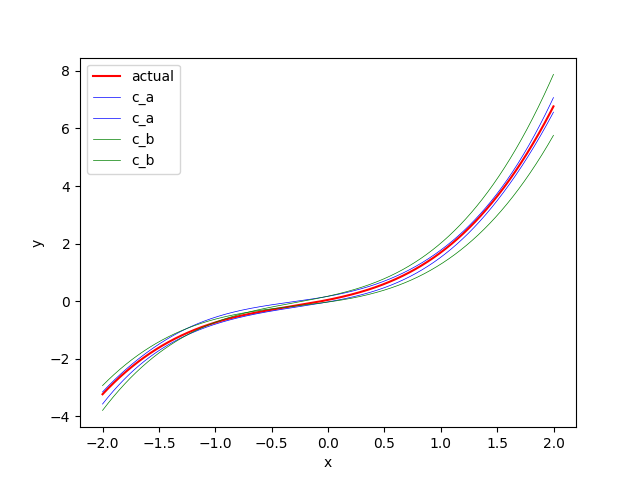
\includegraphics[width=8cm]{../plots/ex3-2.png}
			\centering
			\caption{The actual curve together with the two confidence bands.}
		\end{figure}
	\end{soln}

	\item\label{ex:3.3} Gauss-Markov theorem:
	\begin{enumerate}
		\item Prove the Gauss-Markov theorem: the least squares
		estimate of a parameter $a^T\beta$ has variance no bigger
		than that of any other linear unbiased estimate of $a^T\beta$.

		\item The matrix inequality $\BB\preceq\AA$ holds if $\AA-\BB$
		is positive semidefinite. Show that if $\hat\VV$ is the variance-covariance
		matrix of the least squares estimate $\beta$ and $\tilde\VV$ is the
		variance-covariance matrix of any other linear unbiased estimate, then
		$\hat\VV\preceq\tilde\VV$.
	\end{enumerate} 

	\begin{soln}
		\begin{enumerate}
			\item Let $\hat\beta=(\XX^T\XX)^{-1}\XX^T\yy$ be the least squares
			estimate and consider the estimator of $a^T\beta$ to be
			\[\hat\theta=a^T\hat\beta=\cc_0^T\yy.\]
			Now consider any other unbiased linear estimator $\tilde\theta=\cc^T\yy$ of
			$a^T\beta$; i.e., $E[\cc^T\yy]=a^T\beta$.
			We write $\cc^T=\cc_0^T+d^T$ for some $d$ and we have:
			\begin{equation}
				\begin{split}
					E[\tilde\theta] &= E[(\cc_0^T+d^T)\yy] \\
					&=E[a^T(\XX^T\XX)^{-1}\XX^T\yy + d^T\yy] \\
					&=a^T\beta + d^TE[\yy] \\
					&=a^T\beta + d^T\XX\beta  
				\end{split}
			\end{equation}
			From which, we conclude that \[d^T\XX=0\].

			We now compute the variance of $\tilde\theta$:
			\begin{equation}
				\begin{split}
					\Var[\tilde\theta] &= \Var[\cc^T\yy] \\
					&= \cc^T\Var[\yy]\cc \\
					&= \sigma^2\cc^T\cc \\
					&= \sigma^2(\cc_0^T+d^T)(\cc_0+d) \\
					&= \sigma^2(a^T(\XX^T\XX)^{-1}\XX^T+d^T)(\XX(\XX^T\XX)^{-1}a+d) \\
					&= \sigma^2a^T(\XX^T\XX)^{-1} a + \sigma^2d^Td \\
					&= a^T\sigma^2(\XX^T\XX)^{-1}a + \sigma^2d^Td \\
					&= a^T\Var[\hat\beta]a + \sigma^2d^Td \\
					&= \Var[\hat\theta] + \sigma^2\|d\|^2 \\
					&\ge \Var[\hat\theta].
				\end{split}
			\end{equation}

			\item We can show that this extends to the whole variance-covariance matrix.
			Letting the above $a=I$ the identity matrix and $d=\DD$ any $(p+1)\times(p+1)$
			matrix, we get that 
			\begin{equation}
				\begin{split}
					\Var[\tilde\beta] &= \Var[\hat\beta] + \sigma^2\DD^T\DD
				\end{split}
			\end{equation}
			Therefore, $\Var[\hat\beta]-\Var[\tilde\beta] = \sigma^2\DD^T\DD$ is 
			a Gram matrix and therefore positive-semidefinite.
		\end{enumerate}

		\paragraph{Note.} Another way of stating the Gauss-Markov theorem is that 
		the least squares estimator $\hat\beta$ is \emph{BLUE}: best linear
		unbiased estimator.
	\end{soln}

	\item\label{ex:3.4} Show how the vector of least squares coefficients can 
	be obtained from a single pass of the Gram-Schmidt procedure (Algorithm 3.1).
	Represent your solution in terms of the QR decomposition of $\XX$.

	\begin{soln}
		After having computed the residual vectors $\zz_j$ using Gram-Schmidt, it is straightforward
		to compute the least squares coefficients, by computing
		\[\hat\beta_j=\frac{\ip{\zz_j}{\yy}}{\ip{\zz_j}{\zz_j}}.\]

		In other words, $\hat\beta=(\DD\RR)^{-1}\ZZ^T\yy$ and
		\begin{equation}
			\begin{split}
				\hat\beta &= (\DD\RR)^{-1}\ZZ^T\yy \\
				&= \RR^{-1}\DD^{-1}\ZZ^T\yy \\
				&= \RR^{-1}\QQ^T\yy
			\end{split}
		\end{equation}
	\end{soln}

	\item\label{ex:3.5} Consider the ridge regression problem (3.41). Show that 
	this problem is equivalent to the problem
	\begin{equation}
		\hat\beta^c = \argmin_{\beta^c}\left\{\sum_{i=1}^N\left[y_i-\beta_0^c-\sum_{j=1}^p(x_{ij}-\bar{x}_j)\beta_j^c\right]^2 + \lambda\sum_{j=1}^p{\beta_j^c}^2\right\}.
		\tag{3.85}
	\end{equation}
	Give the correspondence between $\beta^c$ and the original $\beta$ in (3.41).
	Characterize the solution to this modified criterion. Show that a similar
	result holds for the lasso.

	Recall that (3.41) is
	\begin{equation}
		\hat\beta^\ridge = \argmin_{\beta}\left\{\sum_{i=1}^N\left[y_i-\beta_0-\sum_{j=1}^px_{ij}\beta_j\right]^2 + \lambda\sum_{j=1}^p\beta_j^2\right\}.
		\tag{3.41}
	\end{equation}

	\begin{soln}
		Considering for a second the case where $p=1$, observe that by 
		centering the $x_i$, we do not modify $\beta_1$ since $\beta_1$
		estimates the slope and in both cases, the slope remains the same.
		On the other hand, affects the intercept of the line, and hence 
		$\beta_0$. Moreover, assuming that the model is linear,
		the training data $(y_i,x_i-\bar x)$ would give the same model as 
		the training data $(y_i+\bar y,x_i)$, since both data fall on the 
		same line.

		In the case of Ridge Regression, we do not attempt to constrain the
		intercept, hence $\beta_0$ is free to be picked as the intercept of 
		the line.

		In the case where $p=2$, we shift the dependent variables towards some 
		line, again without affecting the normal vector of the plane, only its
		intercept. Similarly, this shift is equivalent to shifting all the
		$y_i$ by a constant amount.

		This idea generalizes to $p$ dimensions. As a result, Ridge regression 
		both with and without centering gives us the same prediction $\beta_j$,
		albeit with a possibly different $\beta_0$.

		Observe that the above analysis \emph{assumes} that the true model is indeed 
		linear.

		A similar result holds for any other penalty function that does not take
		into account the intercept $\beta_0$, hence also for Lasso.
	\end{soln}

	\item\label{ex:3.6} Show that the ridge regression estimate is the mean 
	(and mode) of the posterior distribution, under a Gaussian prior
	$\beta\sim N(0,\tau\II)$ and Gaussian sampling model 
	$\yy\sim N(\XX\beta,\sigma^2\II)$. Find the relationship between the 
	regularization parameter $\lambda$ in the ridge formula, and the variances 
	$\tau$ and $\sigma^2$.

	\begin{soln}
		An answer can be found at
		\footnote[1]
		{\url{https://statisticaloddsandends.wordpress.com/2018/12/29/bayesian-interpretation-of-ridge-regression/}}.

		We first note that
		$\beta\sim N(0,\tau\II)$ and
		$\yy|\beta\sim N(\XX\beta,\sigma^2\II)$ hence the evidence $\yy$
		follows the distribution $\yy\sim N(0,\sigma^2\II+\XX^T\XX\tau)$.
		As usual, the evidence in Bayes Theorem is just a normalization factor 
		and can be ignored. Moreover, we consider $\XX$ to be fixed so the 
		only randomness in the systmem is through $\beta$ and $\yy$. We have 
		\[p(\beta)\varpropto \exp\left[-\frac{1}{2\tau}\|\beta\|^2\right]\]
		and
		\[p(\yy|\beta)\varpropto \exp\left[-\frac{1}{2\sigma^2}(\yy-\XX\beta)^T(\yy-\XX\beta)\right].\]

		We then have
		\begin{equation}
			\begin{split}
				p(\beta|\yy) & \varpropto p(\beta)\cdot p(\yy|\beta) \\
				&\varpropto \exp\left[-\frac{1}{2\tau}\|\beta\|^2-\frac{1}{2\sigma^2}(\yy-\XX\beta)^T(\yy-\XX\beta)\right]
			\end{split}
		\end{equation}

		We can now compute the mode of the posterior as
		\begin{equation}
			\begin{split}
				\argmax_\beta p(\beta|\yy) &=
					\argmax_\beta \exp\left[-\frac{1}{2\tau}\|\beta\|^2-\frac{1}{2\sigma^2}(\yy-\XX\beta)^T(\yy-\XX\beta)\right] \\
					&= \argmin_\beta \exp\left[\frac{1}{2\tau}\|\beta\|^2+\frac{1}{2\sigma^2}(\yy-\XX\beta)^T(\yy-\XX\beta)\right] \\
					&= \argmin_\beta \left(\frac{1}{2\tau}\|\beta\|^2+\frac{1}{2\sigma^2}(\yy-\XX\beta)^T(\yy-\XX\beta)\right) \\
					&= \argmin_\beta \left(\frac{\sigma^2}{\tau}\|\beta\|^2+(\yy-\XX\beta)^T(\yy-\XX\beta)\right) \\
					&= \RSS\left(\frac{\sigma^2}{\tau},\beta\right),
			\end{split}
		\end{equation}
		where, clearly, the last line is the ridge regression estimate.

		\paragraph{Observations.}
		\begin{enumerate}
			\item Note that $\beta$ is centered at 0
			so, intuitively, $\beta$ is more likely to be close to 0,
			especially for small enough variance $\tau$. As a result,
			Ridge is more biased towards zero. This makes sense since Ridge 
			imposes penalty to any variable that is further from 0. At the 
			extreme case, where $\tau = 0^+$, there is no variance at all in 
			which case, Ridge penalizes infinitely the coefficients and it only 
			permits the $0$ as a result.

			\item At the opposite end, if $\tau=\infty$ or $\sigma=0$, the ridge 
			estimate becomes the least squares estimate since there is no penalty.
			As a result, the least squares estimate is the mode of the posterior 
			when the prior is almost uniform or when $\yy=\XX\beta$ always.
		\end{enumerate}
	\end{soln}
\end{enumerate}


\end{document}


